\section{Preliminary}
\label{sec:preliminary}


\subsection{Retrieval Heads and Sparse Heads}
\label{subsec:attn_mechanism}

\paragraph{Retrieval Heads and FA}
Retrieval heads are a class of attention heads specialized in capturing contextually relevant tokens from long sequences, enabling modern LLMs to operate effectively in long-context processing tasks~\citep{wu2024retrieval}.
In practice, retrieval heads typically adopt the standard FA computation mode.
Given the Query ($Q$), Key ($K$), and Value ($V$) states, the computation of FA is :
\begin{equation}
\mathcal{O}_{r}=\mathrm{Softmax}\!\left(QK^{\top}\right)V,
\label{equ:dot_attention}
\end{equation}
where we omit the scaling factor for simplicity.

\paragraph{Sparse Heads and SA}
Compared to the retrieval heads, sparse heads reduce computational cost by leveraging SA mode, which retains only a fraction of the most relevant $K$ and $V$ (e.g., $20\%$ of key and value states).
The computation of SA can be defined as:
\begin{equation}
\mathcal{O}_{s}=\mathrm{Softmax}\!\left(Q\tilde{K}^{\top}\right)\tilde{V},
\label{equ:sparse_attention}
\end{equation}
where $\tilde{K}$ and $\tilde{V}$ are partial elements in $K$ and $V$.

\paragraph{Hybrid Head Mechanism}
While SA substantially reduces computation, it may lead to performance degradation~\citep{lu2025moba}.
To balance efficiency and performance, recent methods adopt a \emph{hybrid heads} design that mixes retrieval and sparse heads within the same model~\citep{xiaoduoattention2025,yu2025sliding,bhaskar2025cache}.
Specifically, for a Transformer with $\mathrm{L}$ layers and $\mathrm{H}$ key--value heads per layer\footnote{Here we adopt grouped query attention (GQA)~\citep{ainslie2023gqa} definition instead of multi-head attention (MHA), as GQA is widely used in modern LLM architectures.}, the $h$-th head in the $\ell$-th layer is assigned a computation type: $\pi^{(\ell, h)} \in \{\text{FA}, \text{SA}\}$, and the final output per layer ($\mathbf{O}^{(\ell)}$) can be written as: 
\begin{equation}
\left\{
\begin{aligned}
& \mathbf{O}^{(\ell)} =
\mathrm{Concat}\!\left(
\mathcal{O}^{(\ell,1)},
\mathcal{O}^{(\ell,2)},
\dots,
\mathcal{O}^{(\ell,\mathrm{H})}
\right),\\
& \mathcal{O}^{(\ell,h)} =
\begin{cases}
\mathcal{O}_{r}, & \pi^{(\ell, h)}=\text{FA},\\
\mathcal{O}_{s}, & \pi^{(\ell, h)}=\text{SA},
\end{cases}
\end{aligned}
\right.
\label{equ:hybrid_concat}
\end{equation}


\begin{figure}[t]
  \centering
    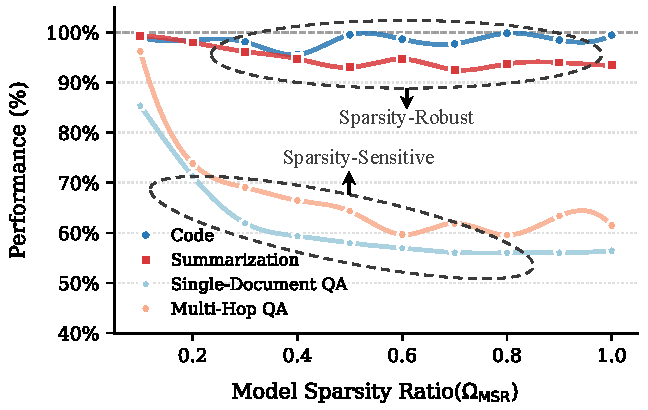
\includegraphics[width=\linewidth]{figures/per_task_performance_1.pdf}
     \caption{Trend of model performance as the hybrid model sparsity ratio ($\mathbf{\Omega_{MSR}}$) increases. We report model performance as a relative percentage score with respect to that of FA.}
  \label{fig:per_task_performance}
\end{figure}

\begin{figure*}[t]
\centering
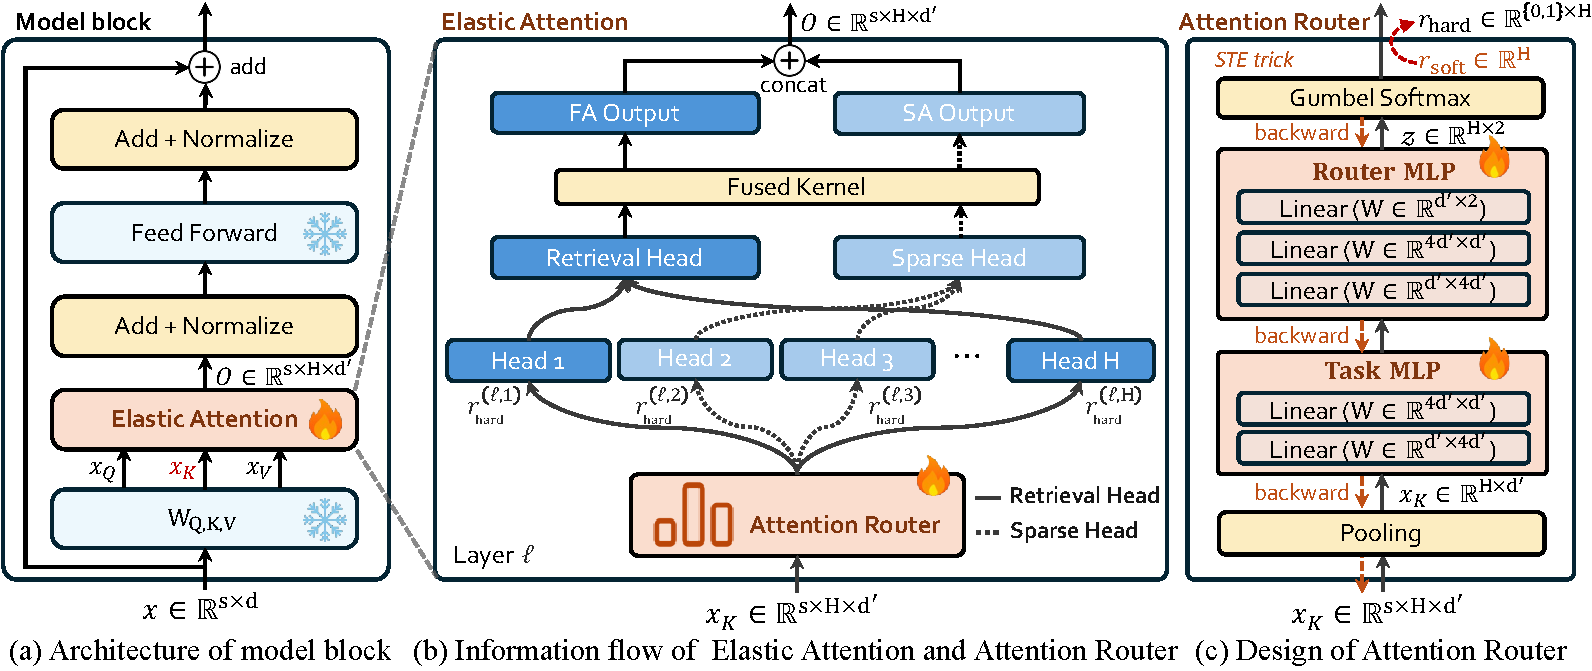
\includegraphics[width=0.95\linewidth]{figures/method_main.pdf}
\caption{Illustration of our proposed Elastic Attention. (a) shows the adapted model block with frozen backbone parameters; (b) details the dynamic assignment of heads via the Attention Router module; (c) presents the lightweight design of the Attention Router.}
\label{fig:method_main}
\end{figure*}

\paragraph{Sparsity Ratio Computation}
Under the hybrid-head mechanism, given a model $f_{\theta}$, we define two types of model sparsity ratios from two perspectives: (1) the proportion of sparse attention heads, and (2) the proportion of tokens attended to by those heads.

\begin{definition}[Model Sparsity Ratio, $\Omega_{\mathrm{MSR}}$]
$\mathbf{\Omega_{\mathrm{MSR}}}$ measures the fraction of sparse heads in the model:
\begin{equation}
\Omega_{\mathrm{MSR}}(f_{\theta})
= \frac{1}{\mathrm{H}}\frac{1}{\mathrm{L}}
\sum_{h=1}^{\mathrm{H}}\sum_{l=1}^{\mathrm{L}}
\mathbb{I}\!\left[\pi^{(\ell, h)}=\mathrm{SA}\right],
\end{equation}
where $\mathbb{I}[\cdot]$ is the indicator function.
\end{definition}

\begin{definition}[Effective Sparsity Ratio, $\Omega_{\mathrm{ESR}}$]
$\mathbf{\Omega_{\mathrm{ESR}}}$ measures the effective sparsity of the entire model, taking both the sparse heads and their corresponding sparsity patterns into account. It can be calculated as:
\begin{equation}
\Omega_{\mathrm{ESR}}(f_{\theta})
=
\frac{1}{\mathrm{H}}
\frac{1}{\mathrm{L}}
\sum_{h=1}^{\mathrm{H}}
\sum_{\ell=1}^{\mathrm{L}}
\rho^{(\mathrm{\ell}, h)},
\end{equation}
where $\rho^{(\ell, h)} \in [0,1)$ denotes the pruning ratio of each head, with $\rho^{(\ell, h)}=0$ for heads with FA, since no tokens are pruned, and $\rho^{(\ell, h)}=\rho_{\mathrm{SA}}$ for heads with SA\footnote{Different SA strategies correspond to specific $\rho_{\mathrm{SA}}$, e.g., if SA only attends to 10\% tokens along the sequence dimension, then $\rho_{\mathrm{SA}}=0.9$, meaning that 90\% of tokens are pruned.}.
\end{definition}

\subsection{Impact of $\mathbf{\Omega_\mathrm{MSR}}$ on Downstream Tasks}
\label{subsec:deployment_sparisity}
While existing hybrid head mechanisms have achieved strong performance–efficiency trade-offs, they suffer from a critical limitation: \emph{the $\mathit{\Omega_\mathit{MSR}}$ is fixed at inference time, and its relationship with downstream task performance remains unexplored.}
In this section, we investigate the impact of varying $\Omega_\mathrm{MSR}$ on different downstream tasks.

\paragraph{Settings}
We experiment with the Llama3.1-8B-Instruct model~\citep{grattafiori2024llama} and follow \citet{wu2024retrieval} to identify retrieval heads in the model and rank them by their activation frequency.
Based on this ranking, we progressively replace retrieval heads with sparse heads, thereby increasing the $\Omega_\mathrm{MSR}$.
We evaluate the above resulting model on LongBench~\citep{bai2024longbench}, which consists of 6 distinct long-context downstream tasks.
For different values of $\Omega_\mathrm{MSR}$, we report the model performance as a percentage relative to that of the backbone model (full FA).
For instance, at an $\Omega_\mathrm{MSR}=20\%$, the resulting model may achieve 73.85\% of the backbone model's performance ($\Omega_\mathrm{MSR}=0\%$).
We provide background of retrieval head identification and implementation details in Appendix~\ref{appendix:preliminary_settings}.

\paragraph{Results}
As shown in Figure~\ref{fig:per_task_performance}, the tasks can be broadly categorized into two categories. 
The first category, which we refer to as \emph{\textbf{sparsity-robust tasks}}, exhibits performance that is largely insensitive to changes in $\Omega_\mathrm{MSR}$. 
This is because these tasks can be solved using only coarse-grained contextual information, e.g., summarization.
The second category, \emph{\textbf{sparsity-sensitive tasks}}, shows a sharp decline in performance once $\Omega_\mathrm{MSR}$ exceeds a certain threshold. 
Such tasks require retrieving fine-grained evidence from the context to produce accurate outputs, as is typical in question-answering tasks.
Therefore, \emph{regardless of the number of task types, they can all be mapped into one of these two categories}. 
Under this setting, the model only needs to determine whether a task requires fine-grained information and then apply the corresponding attention computation mode accordingly.
